\documentclass[aspectratio=169]{beamer}
\usepackage{tikz}
\usetikzlibrary{arrows.meta,bending,positioning,calc}
\usepackage[T1]{fontenc}
\usepackage{lmodern}

\usetheme{default}
\setbeamertemplate{navigation symbols}{}
\setbeamercolor{frametitle}{fg=white,bg=blue!60!black}
\setbeamercolor{background canvas}{bg=white}
\setbeamerfont{frametitle}{series=\bfseries,size=\normalsize}

\tikzset{
  st/.style={
    circle, draw=blue!70!black, fill=blue!10,
    minimum size=10mm, font=\small\bfseries, inner sep=0pt
  },
  % Self-loop style: thin gray arcs with min distance so they don't collapse
  sl/.style={
    -{Stealth[scale=0.55]}, very thin, gray!70!black,
    min distance=9mm, looseness=7
  },
  % Inter-state transition style: thick blue arrows
  tr/.style={
    -{Stealth[scale=0.75]}, thick, blue!80!black
  },
  % Label style: tiny monospace with white opaque background
  lbl/.style={
    font=\tiny\ttfamily, inner sep=1.5pt,
    fill=white, fill opacity=0.88, text opacity=1,
    rounded corners=1pt
  },
}

% Angle-to-label-anchor mapping (consistent across all states):
%   BEACON_REQ  -> out=75,  in=105  -> above
%   ASSOC_REQ   -> out=30,  in=60   -> above right  (when self-loop)
%   REJOIN_TC   -> out=345, in=15   -> right
%   REJOIN_SEC  -> out=300, in=330  -> below right
%   REQ_TCLK    -> out=255, in=285  -> below         (when self-loop)
%   REQ_NWK     -> out=210, in=240  -> below left    (when self-loop)
%   VER_TCLK    -> out=165, in=195  -> left           (when self-loop)
%   VER_GKEY    -> out=120, in=150  -> above left    (when self-loop)

\begin{document}

% ============================================================
% LEGEND
% ============================================================
\begin{frame}{Abbreviation Legend}
\small
\begin{columns}[t]
\column{0.44\textwidth}
  \textbf{Inputs (Stimulus)}\\[5pt]
  \begin{tabular}{@{}ll@{}}
    \texttt{BEACON\_REQ}  & \texttt{MAC\_BEACON\_REQUEST}           \\[2pt]
    \texttt{ASSOC\_REQ}   & \texttt{MAC\_ASSOCIATION\_REQUEST}      \\[2pt]
    \texttt{REJOIN\_TC}   & \texttt{NWK\_REJOIN\_REQUEST\_TC}       \\[2pt]
    \texttt{REJOIN\_SEC}  & \texttt{NWK\_REJOIN\_REQUEST\_SECURE}   \\[2pt]
    \texttt{REQ\_TCLK}    & \texttt{APS\_REQUEST\_TCLK}             \\[2pt]
    \texttt{REQ\_NWK}     & \texttt{APS\_REQUEST\_NWK\_KEY}         \\[2pt]
    \texttt{VER\_TCLK}    & \texttt{APS\_VERIFY\_TCLK}              \\[2pt]
    \texttt{VER\_GKEY}    & \texttt{APS\_VERIFY\_GLOBAL\_KEY}       \\
  \end{tabular}

\column{0.56\textwidth}
  \textbf{Outputs (Response)}\\[5pt]
  \begin{tabular}{@{}ll@{}}
    \texttt{BEACON}       & \texttt{MAC\_BEACON(assoc\_permit=1)}             \\[2pt]
    \texttt{T.NWK+ASSOC}  & \texttt{TRANSPORT\_NWK + ASSOC\_RESP(0)}          \\[2pt]
    \texttt{EMPTY}        & \texttt{EMPTYRESPONSE}                             \\[2pt]
    \texttt{REJ.FAIL}     & \texttt{NWK\_REJOIN\_RESPONSE\_FAILURE(2)}         \\[2pt]
    \texttt{REJ.OK}       & \texttt{NWK\_REJOIN\_RESPONSE\_SUCCESS}            \\[2pt]
    \texttt{T.TCLK}       & \texttt{APS\_CMD\_TRANSPORT\_TC\_LINK\_KEY}        \\[2pt]
    \texttt{ACK}          & \texttt{APS\_ACK}                                  \\[2pt]
    \texttt{CONF.KEY}     & \texttt{APS\_CONFIRM\_KEY(status=0)}               \\[2pt]
    \texttt{T.NWK}        & \texttt{APS\_CMD\_TRANSPORT\_NWK\_KEY}             \\[2pt]
    \texttt{ASSOC.RESP}   & \texttt{MAC\_ASSOCIATION\_RESPONSE(status=0)}      \\
  \end{tabular}
\end{columns}
\end{frame}

% ============================================================
% HYP 1  --  1 state, all 8 transitions are self-loops
% ============================================================
\begin{frame}{Hypothesis 1 \textemdash{} 1 State}
\centering
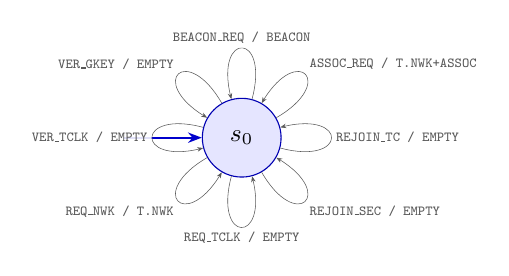
\begin{tikzpicture}[>=Stealth]
  % Initial arrow drawn manually
  \node[st] (s0) at (0,0) {$s_0$};
  \draw[tr] (-1.5,0) -- (s0);

  \path (s0) edge[sl,out=75, in=105] node[lbl,above]       {BEACON\_REQ / BEACON}       (s0);
  \path (s0) edge[sl,out=30, in=60]  node[lbl,above right] {ASSOC\_REQ / T.NWK+ASSOC}   (s0);
  \path (s0) edge[sl,out=345,in=15]  node[lbl,right]       {REJOIN\_TC / EMPTY}          (s0);
  \path (s0) edge[sl,out=300,in=330] node[lbl,below right] {REJOIN\_SEC / EMPTY}         (s0);
  \path (s0) edge[sl,out=255,in=285] node[lbl,below]       {REQ\_TCLK / EMPTY}           (s0);
  \path (s0) edge[sl,out=210,in=240] node[lbl,below left]  {REQ\_NWK / T.NWK}            (s0);
  \path (s0) edge[sl,out=165,in=195] node[lbl,left]        {VER\_TCLK / EMPTY}           (s0);
  \path (s0) edge[sl,out=120,in=150] node[lbl,above left]  {VER\_GKEY / EMPTY}           (s0);
\end{tikzpicture}
\end{frame}

% ============================================================
% HYP 2  --  3 states
%   s0 --(ASSOC_REQ)--> s1   s0 --(REQ_NWK)--> s1
%   s1 --(VER_GKEY)-->  s2
% ============================================================
\begin{frame}{Hypothesis 2 \textemdash{} 3 States}
\centering
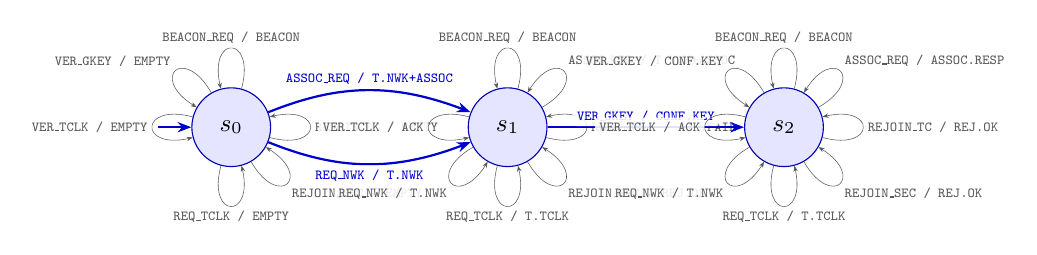
\begin{tikzpicture}[scale=0.78,>=Stealth]
  \node[st] (s0) at (0,0)   {$s_0$};
  \node[st] (s1) at (4.5,0) {$s_1$};
  \node[st] (s2) at (9,0)   {$s_2$};
  \draw[tr] (-1.2,0) -- (s0);

  %% ---- s0  (6 self-loops) ----
  \path (s0) edge[sl,out=75, in=105] node[lbl,above]       {BEACON\_REQ / BEACON}   (s0);
  \path (s0) edge[sl,out=345,in=15]  node[lbl,right]       {REJOIN\_TC / EMPTY}     (s0);
  \path (s0) edge[sl,out=300,in=330] node[lbl,below right] {REJOIN\_SEC / EMPTY}    (s0);
  \path (s0) edge[sl,out=255,in=285] node[lbl,below]       {REQ\_TCLK / EMPTY}      (s0);
  \path (s0) edge[sl,out=165,in=195] node[lbl,left]        {VER\_TCLK / EMPTY}      (s0);
  \path (s0) edge[sl,out=120,in=150] node[lbl,above left]  {VER\_GKEY / EMPTY}      (s0);

  %% ---- s0 -> s1 (2 transitions) ----
  \path (s0) edge[tr,bend left=22]  node[lbl,above] {ASSOC\_REQ / T.NWK+ASSOC} (s1);
  \path (s0) edge[tr,bend right=22] node[lbl,below] {REQ\_NWK / T.NWK}         (s1);

  %% ---- s1  (7 self-loops) ----
  \path (s1) edge[sl,out=75, in=105] node[lbl,above]       {BEACON\_REQ / BEACON}    (s1);
  \path (s1) edge[sl,out=30, in=60]  node[lbl,above right] {ASSOC\_REQ / T.NWK+ASSOC}(s1);
  \path (s1) edge[sl,out=345,in=15]  node[lbl,right]       {REJOIN\_TC / REJ.FAIL}   (s1);
  \path (s1) edge[sl,out=300,in=330] node[lbl,below right] {REJOIN\_SEC / REJ.OK}    (s1);
  \path (s1) edge[sl,out=255,in=285] node[lbl,below]       {REQ\_TCLK / T.TCLK}     (s1);
  \path (s1) edge[sl,out=210,in=240] node[lbl,below left]  {REQ\_NWK / T.NWK}        (s1);
  \path (s1) edge[sl,out=165,in=195] node[lbl,left]        {VER\_TCLK / ACK}         (s1);

  %% ---- s1 -> s2 ----
  \path (s1) edge[tr] node[lbl,above] {VER\_GKEY / CONF.KEY} (s2);

  %% ---- s2  (8 self-loops) ----
  \path (s2) edge[sl,out=75, in=105] node[lbl,above]       {BEACON\_REQ / BEACON}    (s2);
  \path (s2) edge[sl,out=30, in=60]  node[lbl,above right] {ASSOC\_REQ / ASSOC.RESP} (s2);
  \path (s2) edge[sl,out=345,in=15]  node[lbl,right]       {REJOIN\_TC / REJ.OK}     (s2);
  \path (s2) edge[sl,out=300,in=330] node[lbl,below right] {REJOIN\_SEC / REJ.OK}    (s2);
  \path (s2) edge[sl,out=255,in=285] node[lbl,below]       {REQ\_TCLK / T.TCLK}     (s2);
  \path (s2) edge[sl,out=210,in=240] node[lbl,below left]  {REQ\_NWK / T.NWK}        (s2);
  \path (s2) edge[sl,out=165,in=195] node[lbl,left]        {VER\_TCLK / ACK}         (s2);
  \path (s2) edge[sl,out=120,in=150] node[lbl,above left]  {VER\_GKEY / CONF.KEY}    (s2);
\end{tikzpicture}
\end{frame}

% ============================================================
% HYP 3  --  4 states
%   s0 --(ASSOC_REQ)--> s1    s0 --(REQ_NWK)--> s3
%   s1 --(VER_GKEY)-->  s2    s3 --(ASSOC_REQ)-> s1
% ============================================================
\begin{frame}{Hypothesis 3 \textemdash{} 4 States}
\centering
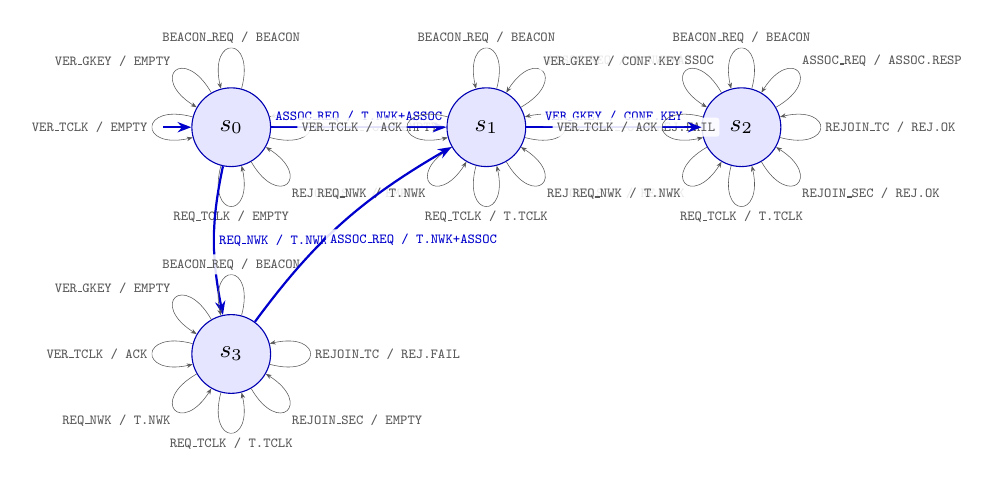
\begin{tikzpicture}[scale=0.72,>=Stealth]
  \node[st] (s0) at (0,0)   {$s_0$};
  \node[st] (s1) at (4.5,0) {$s_1$};
  \node[st] (s2) at (9,0)   {$s_2$};
  \node[st] (s3) at (0,-4)  {$s_3$};
  \draw[tr] (-1.2,0) -- (s0);

  %% ---- s0  (6 self-loops) ----
  \path (s0) edge[sl,out=75, in=105] node[lbl,above]       {BEACON\_REQ / BEACON}   (s0);
  \path (s0) edge[sl,out=345,in=15]  node[lbl,right]       {REJOIN\_TC / EMPTY}     (s0);
  \path (s0) edge[sl,out=300,in=330] node[lbl,below right] {REJOIN\_SEC / EMPTY}    (s0);
  \path (s0) edge[sl,out=255,in=285] node[lbl,below]       {REQ\_TCLK / EMPTY}      (s0);
  \path (s0) edge[sl,out=165,in=195] node[lbl,left]        {VER\_TCLK / EMPTY}      (s0);
  \path (s0) edge[sl,out=120,in=150] node[lbl,above left]  {VER\_GKEY / EMPTY}      (s0);

  %% ---- s0 -> s1, s0 -> s3 ----
  \path (s0) edge[tr]            node[lbl,above]      {ASSOC\_REQ / T.NWK+ASSOC} (s1);
  \path (s0) edge[tr,bend right=12] node[lbl,right]   {REQ\_NWK / T.NWK}         (s3);

  %% ---- s1  (7 self-loops) ----
  \path (s1) edge[sl,out=75, in=105] node[lbl,above]       {BEACON\_REQ / BEACON}     (s1);
  \path (s1) edge[sl,out=30, in=60]  node[lbl,above right] {ASSOC\_REQ / T.NWK+ASSOC} (s1);
  \path (s1) edge[sl,out=345,in=15]  node[lbl,right]       {REJOIN\_TC / REJ.FAIL}    (s1);
  \path (s1) edge[sl,out=300,in=330] node[lbl,below right] {REJOIN\_SEC / REJ.OK}     (s1);
  \path (s1) edge[sl,out=255,in=285] node[lbl,below]       {REQ\_TCLK / T.TCLK}      (s1);
  \path (s1) edge[sl,out=210,in=240] node[lbl,below left]  {REQ\_NWK / T.NWK}         (s1);
  \path (s1) edge[sl,out=165,in=195] node[lbl,left]        {VER\_TCLK / ACK}          (s1);

  %% ---- s1 -> s2 ----
  \path (s1) edge[tr] node[lbl,above] {VER\_GKEY / CONF.KEY} (s2);

  %% ---- s2  (8 self-loops) ----
  \path (s2) edge[sl,out=75, in=105] node[lbl,above]       {BEACON\_REQ / BEACON}    (s2);
  \path (s2) edge[sl,out=30, in=60]  node[lbl,above right] {ASSOC\_REQ / ASSOC.RESP} (s2);
  \path (s2) edge[sl,out=345,in=15]  node[lbl,right]       {REJOIN\_TC / REJ.OK}     (s2);
  \path (s2) edge[sl,out=300,in=330] node[lbl,below right] {REJOIN\_SEC / REJ.OK}    (s2);
  \path (s2) edge[sl,out=255,in=285] node[lbl,below]       {REQ\_TCLK / T.TCLK}     (s2);
  \path (s2) edge[sl,out=210,in=240] node[lbl,below left]  {REQ\_NWK / T.NWK}        (s2);
  \path (s2) edge[sl,out=165,in=195] node[lbl,left]        {VER\_TCLK / ACK}         (s2);
  \path (s2) edge[sl,out=120,in=150] node[lbl,above left]  {VER\_GKEY / CONF.KEY}    (s2);

  %% ---- s3  (7 self-loops) ----
  \path (s3) edge[sl,out=75, in=105] node[lbl,above]       {BEACON\_REQ / BEACON}   (s3);
  \path (s3) edge[sl,out=345,in=15]  node[lbl,right]       {REJOIN\_TC / REJ.FAIL}  (s3);
  \path (s3) edge[sl,out=300,in=330] node[lbl,below right] {REJOIN\_SEC / EMPTY}    (s3);
  \path (s3) edge[sl,out=255,in=285] node[lbl,below]       {REQ\_TCLK / T.TCLK}    (s3);
  \path (s3) edge[sl,out=210,in=240] node[lbl,below left]  {REQ\_NWK / T.NWK}       (s3);
  \path (s3) edge[sl,out=165,in=195] node[lbl,left]        {VER\_TCLK / ACK}        (s3);
  \path (s3) edge[sl,out=120,in=150] node[lbl,above left]  {VER\_GKEY / EMPTY}      (s3);

  %% ---- s3 -> s1 ----
  \path (s3) edge[tr,bend left=12] node[lbl,right,pos=0.4] {ASSOC\_REQ / T.NWK+ASSOC} (s1);
\end{tikzpicture}
\end{frame}

% ============================================================
% HYP 4  --  5 states
%   s0 -> s1 (ASSOC_REQ)    s0 -> s3 (REQ_NWK)
%   s1 -> s2 (VER_GKEY)     s2 -> s4 (REQ_TCLK)
%   s3 -> s1 (ASSOC_REQ)
% ============================================================
\begin{frame}{Hypothesis 4 \textemdash{} 5 States}
\centering
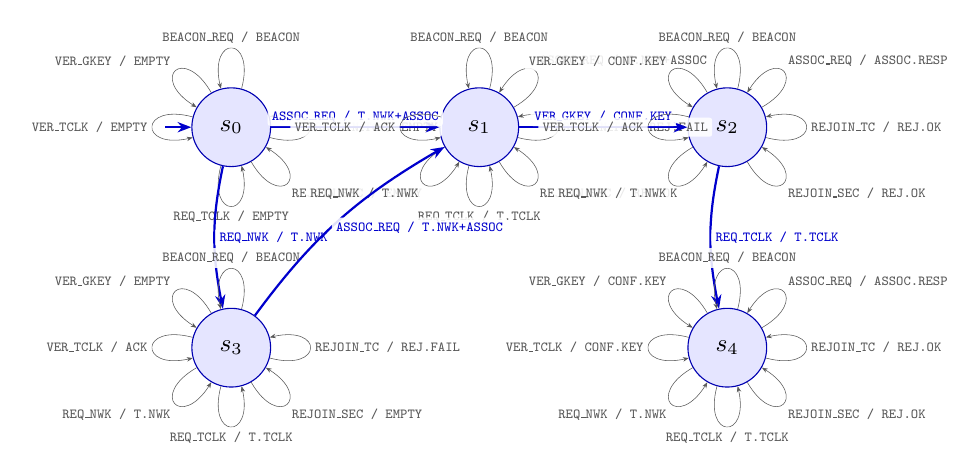
\begin{tikzpicture}[scale=0.70,>=Stealth]
  \node[st] (s0) at (0,0)   {$s_0$};
  \node[st] (s1) at (4.5,0) {$s_1$};
  \node[st] (s2) at (9,0)   {$s_2$};
  \node[st] (s3) at (0,-4)  {$s_3$};
  \node[st] (s4) at (9,-4)  {$s_4$};
  \draw[tr] (-1.2,0) -- (s0);

  %% ---- s0  (6 self-loops) ----
  \path (s0) edge[sl,out=75, in=105] node[lbl,above]       {BEACON\_REQ / BEACON}   (s0);
  \path (s0) edge[sl,out=345,in=15]  node[lbl,right]       {REJOIN\_TC / EMPTY}     (s0);
  \path (s0) edge[sl,out=300,in=330] node[lbl,below right] {REJOIN\_SEC / EMPTY}    (s0);
  \path (s0) edge[sl,out=255,in=285] node[lbl,below]       {REQ\_TCLK / EMPTY}      (s0);
  \path (s0) edge[sl,out=165,in=195] node[lbl,left]        {VER\_TCLK / EMPTY}      (s0);
  \path (s0) edge[sl,out=120,in=150] node[lbl,above left]  {VER\_GKEY / EMPTY}      (s0);

  \path (s0) edge[tr]               node[lbl,above]   {ASSOC\_REQ / T.NWK+ASSOC} (s1);
  \path (s0) edge[tr,bend right=12] node[lbl,right]   {REQ\_NWK / T.NWK}         (s3);

  %% ---- s1  (7 self-loops) ----
  \path (s1) edge[sl,out=75, in=105] node[lbl,above]       {BEACON\_REQ / BEACON}     (s1);
  \path (s1) edge[sl,out=30, in=60]  node[lbl,above right] {ASSOC\_REQ / T.NWK+ASSOC} (s1);
  \path (s1) edge[sl,out=345,in=15]  node[lbl,right]       {REJOIN\_TC / REJ.FAIL}    (s1);
  \path (s1) edge[sl,out=300,in=330] node[lbl,below right] {REJOIN\_SEC / REJ.OK}     (s1);
  \path (s1) edge[sl,out=255,in=285] node[lbl,below]       {REQ\_TCLK / T.TCLK}      (s1);
  \path (s1) edge[sl,out=210,in=240] node[lbl,below left]  {REQ\_NWK / T.NWK}         (s1);
  \path (s1) edge[sl,out=165,in=195] node[lbl,left]        {VER\_TCLK / ACK}          (s1);

  \path (s1) edge[tr] node[lbl,above] {VER\_GKEY / CONF.KEY} (s2);

  %% ---- s2  (7 self-loops, REQ_TCLK -> s4) ----
  \path (s2) edge[sl,out=75, in=105] node[lbl,above]       {BEACON\_REQ / BEACON}    (s2);
  \path (s2) edge[sl,out=30, in=60]  node[lbl,above right] {ASSOC\_REQ / ASSOC.RESP} (s2);
  \path (s2) edge[sl,out=345,in=15]  node[lbl,right]       {REJOIN\_TC / REJ.OK}     (s2);
  \path (s2) edge[sl,out=300,in=330] node[lbl,below right] {REJOIN\_SEC / REJ.OK}    (s2);
  \path (s2) edge[sl,out=210,in=240] node[lbl,below left]  {REQ\_NWK / T.NWK}        (s2);
  \path (s2) edge[sl,out=165,in=195] node[lbl,left]        {VER\_TCLK / ACK}         (s2);
  \path (s2) edge[sl,out=120,in=150] node[lbl,above left]  {VER\_GKEY / CONF.KEY}    (s2);

  \path (s2) edge[tr,bend right=12] node[lbl,right] {REQ\_TCLK / T.TCLK} (s4);

  %% ---- s3  (7 self-loops) ----
  \path (s3) edge[sl,out=75, in=105] node[lbl,above]       {BEACON\_REQ / BEACON}   (s3);
  \path (s3) edge[sl,out=345,in=15]  node[lbl,right]       {REJOIN\_TC / REJ.FAIL}  (s3);
  \path (s3) edge[sl,out=300,in=330] node[lbl,below right] {REJOIN\_SEC / EMPTY}    (s3);
  \path (s3) edge[sl,out=255,in=285] node[lbl,below]       {REQ\_TCLK / T.TCLK}    (s3);
  \path (s3) edge[sl,out=210,in=240] node[lbl,below left]  {REQ\_NWK / T.NWK}       (s3);
  \path (s3) edge[sl,out=165,in=195] node[lbl,left]        {VER\_TCLK / ACK}        (s3);
  \path (s3) edge[sl,out=120,in=150] node[lbl,above left]  {VER\_GKEY / EMPTY}      (s3);

  \path (s3) edge[tr,bend left=12] node[lbl,right,pos=0.45] {ASSOC\_REQ / T.NWK+ASSOC} (s1);

  %% ---- s4  (8 self-loops) ----
  \path (s4) edge[sl,out=75, in=105] node[lbl,above]       {BEACON\_REQ / BEACON}    (s4);
  \path (s4) edge[sl,out=30, in=60]  node[lbl,above right] {ASSOC\_REQ / ASSOC.RESP} (s4);
  \path (s4) edge[sl,out=345,in=15]  node[lbl,right]       {REJOIN\_TC / REJ.OK}     (s4);
  \path (s4) edge[sl,out=300,in=330] node[lbl,below right] {REJOIN\_SEC / REJ.OK}    (s4);
  \path (s4) edge[sl,out=255,in=285] node[lbl,below]       {REQ\_TCLK / T.TCLK}     (s4);
  \path (s4) edge[sl,out=210,in=240] node[lbl,below left]  {REQ\_NWK / T.NWK}        (s4);
  \path (s4) edge[sl,out=165,in=195] node[lbl,left]        {VER\_TCLK / CONF.KEY}    (s4);
  \path (s4) edge[sl,out=120,in=150] node[lbl,above left]  {VER\_GKEY / CONF.KEY}    (s4);
\end{tikzpicture}
\end{frame}

% ============================================================
% HYP 5  --  6 states
%   s0 -> s1 (ASSOC_REQ)    s0 -> s3 (REQ_NWK)
%   s1 -> s2 (VER_GKEY)     s1 -> s5 (REQ_TCLK)  [new!]
%   s2 -> s4 (REQ_TCLK)     s3 -> s1 (ASSOC_REQ)
%   s5 -> s4 (VER_TCLK)     s5 -> s4 (VER_GKEY)
% ============================================================
\begin{frame}{Hypothesis 5 \textemdash{} 6 States}
\centering
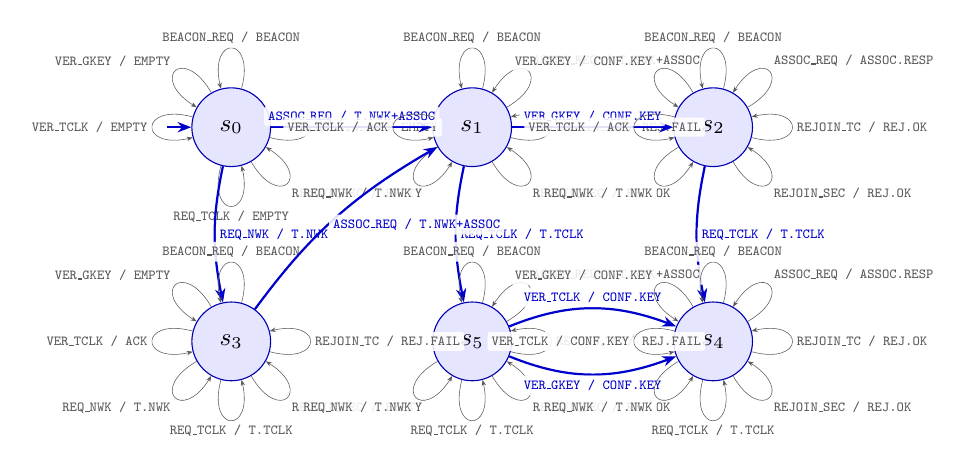
\begin{tikzpicture}[scale=0.68,>=Stealth]
  \node[st] (s0) at (0,0)     {$s_0$};
  \node[st] (s1) at (4.5,0)   {$s_1$};
  \node[st] (s2) at (9,0)     {$s_2$};
  \node[st] (s3) at (0,-4)    {$s_3$};
  \node[st] (s5) at (4.5,-4)  {$s_5$};
  \node[st] (s4) at (9,-4)    {$s_4$};
  \draw[tr] (-1.2,0) -- (s0);

  %% ---- s0  (6 self-loops) ----
  \path (s0) edge[sl,out=75, in=105] node[lbl,above]       {BEACON\_REQ / BEACON}   (s0);
  \path (s0) edge[sl,out=345,in=15]  node[lbl,right]       {REJOIN\_TC / EMPTY}     (s0);
  \path (s0) edge[sl,out=300,in=330] node[lbl,below right] {REJOIN\_SEC / EMPTY}    (s0);
  \path (s0) edge[sl,out=255,in=285] node[lbl,below]       {REQ\_TCLK / EMPTY}      (s0);
  \path (s0) edge[sl,out=165,in=195] node[lbl,left]        {VER\_TCLK / EMPTY}      (s0);
  \path (s0) edge[sl,out=120,in=150] node[lbl,above left]  {VER\_GKEY / EMPTY}      (s0);

  \path (s0) edge[tr]               node[lbl,above]   {ASSOC\_REQ / T.NWK+ASSOC} (s1);
  \path (s0) edge[tr,bend right=12] node[lbl,right]   {REQ\_NWK / T.NWK}         (s3);

  %% ---- s1  (6 self-loops, REQ_TCLK->s5 and VER_GKEY->s2) ----
  \path (s1) edge[sl,out=75, in=105] node[lbl,above]       {BEACON\_REQ / BEACON}     (s1);
  \path (s1) edge[sl,out=30, in=60]  node[lbl,above right] {ASSOC\_REQ / T.NWK+ASSOC} (s1);
  \path (s1) edge[sl,out=345,in=15]  node[lbl,right]       {REJOIN\_TC / REJ.FAIL}    (s1);
  \path (s1) edge[sl,out=300,in=330] node[lbl,below right] {REJOIN\_SEC / REJ.OK}     (s1);
  \path (s1) edge[sl,out=210,in=240] node[lbl,below left]  {REQ\_NWK / T.NWK}         (s1);
  \path (s1) edge[sl,out=165,in=195] node[lbl,left]        {VER\_TCLK / ACK}          (s1);

  \path (s1) edge[tr]               node[lbl,above]  {VER\_GKEY / CONF.KEY} (s2);
  \path (s1) edge[tr,bend right=12] node[lbl,right]  {REQ\_TCLK / T.TCLK}  (s5);

  %% ---- s2  (7 self-loops, REQ_TCLK -> s4) ----
  \path (s2) edge[sl,out=75, in=105] node[lbl,above]       {BEACON\_REQ / BEACON}    (s2);
  \path (s2) edge[sl,out=30, in=60]  node[lbl,above right] {ASSOC\_REQ / ASSOC.RESP} (s2);
  \path (s2) edge[sl,out=345,in=15]  node[lbl,right]       {REJOIN\_TC / REJ.OK}     (s2);
  \path (s2) edge[sl,out=300,in=330] node[lbl,below right] {REJOIN\_SEC / REJ.OK}    (s2);
  \path (s2) edge[sl,out=210,in=240] node[lbl,below left]  {REQ\_NWK / T.NWK}        (s2);
  \path (s2) edge[sl,out=165,in=195] node[lbl,left]        {VER\_TCLK / ACK}         (s2);
  \path (s2) edge[sl,out=120,in=150] node[lbl,above left]  {VER\_GKEY / CONF.KEY}    (s2);

  \path (s2) edge[tr,bend right=12] node[lbl,right] {REQ\_TCLK / T.TCLK} (s4);

  %% ---- s3  (7 self-loops) ----
  \path (s3) edge[sl,out=75, in=105] node[lbl,above]       {BEACON\_REQ / BEACON}   (s3);
  \path (s3) edge[sl,out=345,in=15]  node[lbl,right]       {REJOIN\_TC / REJ.FAIL}  (s3);
  \path (s3) edge[sl,out=300,in=330] node[lbl,below right] {REJOIN\_SEC / EMPTY}    (s3);
  \path (s3) edge[sl,out=255,in=285] node[lbl,below]       {REQ\_TCLK / T.TCLK}    (s3);
  \path (s3) edge[sl,out=210,in=240] node[lbl,below left]  {REQ\_NWK / T.NWK}       (s3);
  \path (s3) edge[sl,out=165,in=195] node[lbl,left]        {VER\_TCLK / ACK}        (s3);
  \path (s3) edge[sl,out=120,in=150] node[lbl,above left]  {VER\_GKEY / EMPTY}      (s3);

  \path (s3) edge[tr,bend left=12] node[lbl,right,pos=0.45] {ASSOC\_REQ / T.NWK+ASSOC} (s1);

  %% ---- s5  (6 self-loops, VER_TCLK->s4 and VER_GKEY->s4) ----
  \path (s5) edge[sl,out=75, in=105] node[lbl,above]       {BEACON\_REQ / BEACON}     (s5);
  \path (s5) edge[sl,out=30, in=60]  node[lbl,above right] {ASSOC\_REQ / T.NWK+ASSOC} (s5);
  \path (s5) edge[sl,out=345,in=15]  node[lbl,right]       {REJOIN\_TC / REJ.FAIL}    (s5);
  \path (s5) edge[sl,out=300,in=330] node[lbl,below right] {REJOIN\_SEC / REJ.OK}     (s5);
  \path (s5) edge[sl,out=255,in=285] node[lbl,below]       {REQ\_TCLK / T.TCLK}      (s5);
  \path (s5) edge[sl,out=210,in=240] node[lbl,below left]  {REQ\_NWK / T.NWK}         (s5);

  \path (s5) edge[tr,bend left=22]  node[lbl,above] {VER\_TCLK / CONF.KEY} (s4);
  \path (s5) edge[tr,bend right=22] node[lbl,below] {VER\_GKEY / CONF.KEY} (s4);

  %% ---- s4  (8 self-loops) ----
  \path (s4) edge[sl,out=75, in=105] node[lbl,above]       {BEACON\_REQ / BEACON}    (s4);
  \path (s4) edge[sl,out=30, in=60]  node[lbl,above right] {ASSOC\_REQ / ASSOC.RESP} (s4);
  \path (s4) edge[sl,out=345,in=15]  node[lbl,right]       {REJOIN\_TC / REJ.OK}     (s4);
  \path (s4) edge[sl,out=300,in=330] node[lbl,below right] {REJOIN\_SEC / REJ.OK}    (s4);
  \path (s4) edge[sl,out=255,in=285] node[lbl,below]       {REQ\_TCLK / T.TCLK}     (s4);
  \path (s4) edge[sl,out=210,in=240] node[lbl,below left]  {REQ\_NWK / T.NWK}        (s4);
  \path (s4) edge[sl,out=165,in=195] node[lbl,left]        {VER\_TCLK / CONF.KEY}    (s4);
  \path (s4) edge[sl,out=120,in=150] node[lbl,above left]  {VER\_GKEY / CONF.KEY}    (s4);
\end{tikzpicture}
\end{frame}

% ============================================================
% HYP 6  --  7 states (final / learned model)
%   s0 -> s1 (ASSOC_REQ)    s0 -> s3 (REQ_NWK)
%   s1 -> s2 (VER_GKEY)     s1 -> s5 (REQ_TCLK)
%   s2 -> s4 (REQ_TCLK)
%   s3 -> s1 (ASSOC_REQ)    s3 -> s6 (REQ_TCLK)  [new!]
%   s5 -> s4 (VER_TCLK)     s5 -> s4 (VER_GKEY)
%   s6 -> s5 (ASSOC_REQ)    [new!]
% ============================================================
\begin{frame}{Hypothesis 6 \textemdash{} 7 States (Final Model)}
\centering
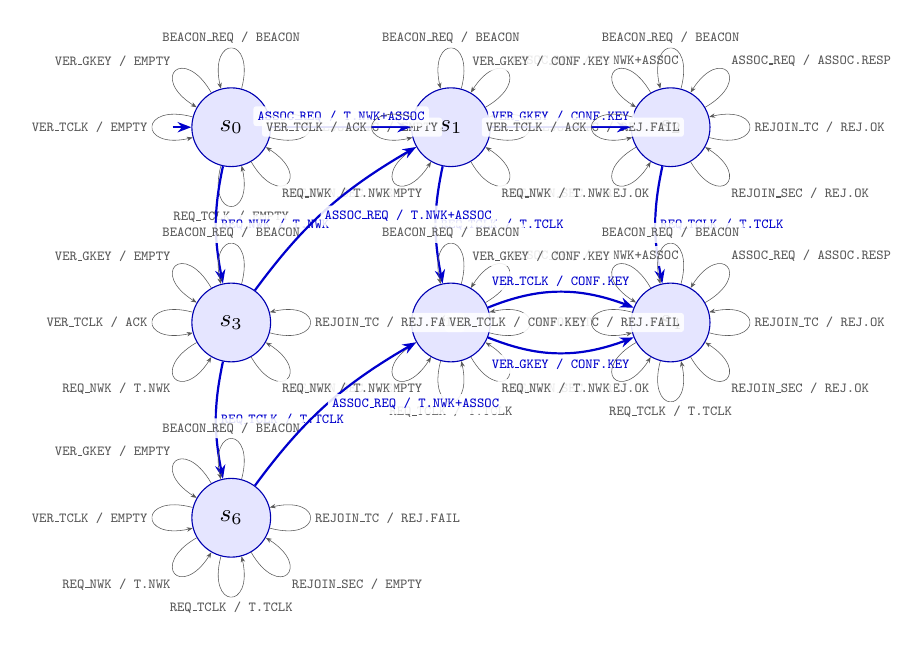
\begin{tikzpicture}[scale=0.62,>=Stealth]
  \node[st] (s0) at (0,0)    {$s_0$};
  \node[st] (s1) at (4.5,0)  {$s_1$};
  \node[st] (s2) at (9,0)    {$s_2$};
  \node[st] (s3) at (0,-4)   {$s_3$};
  \node[st] (s5) at (4.5,-4) {$s_5$};
  \node[st] (s4) at (9,-4)   {$s_4$};
  \node[st] (s6) at (0,-8)   {$s_6$};
  \draw[tr] (-1.2,0) -- (s0);

  %% ---- s0  (6 self-loops) ----
  \path (s0) edge[sl,out=75, in=105] node[lbl,above]       {BEACON\_REQ / BEACON}   (s0);
  \path (s0) edge[sl,out=345,in=15]  node[lbl,right]       {REJOIN\_TC / EMPTY}     (s0);
  \path (s0) edge[sl,out=300,in=330] node[lbl,below right] {REJOIN\_SEC / EMPTY}    (s0);
  \path (s0) edge[sl,out=255,in=285] node[lbl,below]       {REQ\_TCLK / EMPTY}      (s0);
  \path (s0) edge[sl,out=165,in=195] node[lbl,left]        {VER\_TCLK / EMPTY}      (s0);
  \path (s0) edge[sl,out=120,in=150] node[lbl,above left]  {VER\_GKEY / EMPTY}      (s0);

  \path (s0) edge[tr]               node[lbl,above]   {ASSOC\_REQ / T.NWK+ASSOC} (s1);
  \path (s0) edge[tr,bend right=12] node[lbl,right]   {REQ\_NWK / T.NWK}         (s3);

  %% ---- s1  (6 self-loops) ----
  \path (s1) edge[sl,out=75, in=105] node[lbl,above]       {BEACON\_REQ / BEACON}     (s1);
  \path (s1) edge[sl,out=30, in=60]  node[lbl,above right] {ASSOC\_REQ / T.NWK+ASSOC} (s1);
  \path (s1) edge[sl,out=345,in=15]  node[lbl,right]       {REJOIN\_TC / REJ.FAIL}    (s1);
  \path (s1) edge[sl,out=300,in=330] node[lbl,below right] {REJOIN\_SEC / REJ.OK}     (s1);
  \path (s1) edge[sl,out=210,in=240] node[lbl,below left]  {REQ\_NWK / T.NWK}         (s1);
  \path (s1) edge[sl,out=165,in=195] node[lbl,left]        {VER\_TCLK / ACK}          (s1);

  \path (s1) edge[tr]               node[lbl,above]  {VER\_GKEY / CONF.KEY} (s2);
  \path (s1) edge[tr,bend right=12] node[lbl,right]  {REQ\_TCLK / T.TCLK}  (s5);

  %% ---- s2  (7 self-loops, REQ_TCLK -> s4) ----
  \path (s2) edge[sl,out=75, in=105] node[lbl,above]       {BEACON\_REQ / BEACON}    (s2);
  \path (s2) edge[sl,out=30, in=60]  node[lbl,above right] {ASSOC\_REQ / ASSOC.RESP} (s2);
  \path (s2) edge[sl,out=345,in=15]  node[lbl,right]       {REJOIN\_TC / REJ.OK}     (s2);
  \path (s2) edge[sl,out=300,in=330] node[lbl,below right] {REJOIN\_SEC / REJ.OK}    (s2);
  \path (s2) edge[sl,out=210,in=240] node[lbl,below left]  {REQ\_NWK / T.NWK}        (s2);
  \path (s2) edge[sl,out=165,in=195] node[lbl,left]        {VER\_TCLK / ACK}         (s2);
  \path (s2) edge[sl,out=120,in=150] node[lbl,above left]  {VER\_GKEY / CONF.KEY}    (s2);

  \path (s2) edge[tr,bend right=12] node[lbl,right] {REQ\_TCLK / T.TCLK} (s4);

  %% ---- s3  (6 self-loops, ASSOC_REQ->s1 and REQ_TCLK->s6) ----
  \path (s3) edge[sl,out=75, in=105] node[lbl,above]       {BEACON\_REQ / BEACON}   (s3);
  \path (s3) edge[sl,out=345,in=15]  node[lbl,right]       {REJOIN\_TC / REJ.FAIL}  (s3);
  \path (s3) edge[sl,out=300,in=330] node[lbl,below right] {REJOIN\_SEC / EMPTY}    (s3);
  \path (s3) edge[sl,out=210,in=240] node[lbl,below left]  {REQ\_NWK / T.NWK}       (s3);
  \path (s3) edge[sl,out=165,in=195] node[lbl,left]        {VER\_TCLK / ACK}        (s3);
  \path (s3) edge[sl,out=120,in=150] node[lbl,above left]  {VER\_GKEY / EMPTY}      (s3);

  \path (s3) edge[tr,bend left=12]  node[lbl,right,pos=0.45] {ASSOC\_REQ / T.NWK+ASSOC} (s1);
  \path (s3) edge[tr,bend right=12] node[lbl,right]           {REQ\_TCLK / T.TCLK}       (s6);

  %% ---- s5  (6 self-loops, VER_TCLK->s4 and VER_GKEY->s4) ----
  \path (s5) edge[sl,out=75, in=105] node[lbl,above]       {BEACON\_REQ / BEACON}     (s5);
  \path (s5) edge[sl,out=30, in=60]  node[lbl,above right] {ASSOC\_REQ / T.NWK+ASSOC} (s5);
  \path (s5) edge[sl,out=345,in=15]  node[lbl,right]       {REJOIN\_TC / REJ.FAIL}    (s5);
  \path (s5) edge[sl,out=300,in=330] node[lbl,below right] {REJOIN\_SEC / REJ.OK}     (s5);
  \path (s5) edge[sl,out=255,in=285] node[lbl,below]       {REQ\_TCLK / T.TCLK}      (s5);
  \path (s5) edge[sl,out=210,in=240] node[lbl,below left]  {REQ\_NWK / T.NWK}         (s5);

  \path (s5) edge[tr,bend left=22]  node[lbl,above] {VER\_TCLK / CONF.KEY} (s4);
  \path (s5) edge[tr,bend right=22] node[lbl,below] {VER\_GKEY / CONF.KEY} (s4);

  %% ---- s4  (8 self-loops) ----
  \path (s4) edge[sl,out=75, in=105] node[lbl,above]       {BEACON\_REQ / BEACON}    (s4);
  \path (s4) edge[sl,out=30, in=60]  node[lbl,above right] {ASSOC\_REQ / ASSOC.RESP} (s4);
  \path (s4) edge[sl,out=345,in=15]  node[lbl,right]       {REJOIN\_TC / REJ.OK}     (s4);
  \path (s4) edge[sl,out=300,in=330] node[lbl,below right] {REJOIN\_SEC / REJ.OK}    (s4);
  \path (s4) edge[sl,out=255,in=285] node[lbl,below]       {REQ\_TCLK / T.TCLK}     (s4);
  \path (s4) edge[sl,out=210,in=240] node[lbl,below left]  {REQ\_NWK / T.NWK}        (s4);
  \path (s4) edge[sl,out=165,in=195] node[lbl,left]        {VER\_TCLK / CONF.KEY}    (s4);
  \path (s4) edge[sl,out=120,in=150] node[lbl,above left]  {VER\_GKEY / CONF.KEY}    (s4);

  %% ---- s6  (7 self-loops, ASSOC_REQ -> s5) ----
  \path (s6) edge[sl,out=75, in=105] node[lbl,above]       {BEACON\_REQ / BEACON}   (s6);
  \path (s6) edge[sl,out=345,in=15]  node[lbl,right]       {REJOIN\_TC / REJ.FAIL}  (s6);
  \path (s6) edge[sl,out=300,in=330] node[lbl,below right] {REJOIN\_SEC / EMPTY}    (s6);
  \path (s6) edge[sl,out=255,in=285] node[lbl,below]       {REQ\_TCLK / T.TCLK}    (s6);
  \path (s6) edge[sl,out=210,in=240] node[lbl,below left]  {REQ\_NWK / T.NWK}       (s6);
  \path (s6) edge[sl,out=165,in=195] node[lbl,left]        {VER\_TCLK / EMPTY}      (s6);
  \path (s6) edge[sl,out=120,in=150] node[lbl,above left]  {VER\_GKEY / EMPTY}      (s6);

  \path (s6) edge[tr,bend left=12] node[lbl,right,pos=0.5] {ASSOC\_REQ / T.NWK+ASSOC} (s5);
\end{tikzpicture}
\end{frame}

\end{document}
